\documentclass{article}
\usepackage{gonza}
\lfoot{\textcolor{gray2}{Part of the ExaTN LDRD}}

\lstset{language=c++,basicstyle=\footnotesize\ttfamily,
	keywordstyle=\color{blue}\bfseries,frame=shadowbox}

\newcommand{\code}[1]{\texttt{#1}}

\begin{document}
	\begin{center}
		{\LARGE The MERA++ Symbolic Driver}\vspace{0.5cm}\\
		
	{G.~A.}
	
\end{center}

\section{The MERA}
Multiscale Entanglement Renormalization Ansatz (MERA) refers to a class of tensor networks where a linear mapping is repeatedly applied generate a rescaled quantum theory. 
The main meta-parameters specifying MERA networks are: the dimension \code{-d}, number of renormalization layers \code{-l}, the isometry arity \code{-a}, and the periodicity \code{-P}. 
These parameters, along with a geometric tiling, induce an underlying graph structure which fixes the number of physical sites \code{-n}. 
See figure 1(a) for a graphical description the parameters.
The MERA++ symbolic driver \code{merapp} inputs the parameters of the MERA and outputs a string representation of the MERA, or an sRep.

Along with the meta- parameters each tensor of the MERA needs to be specified. 
This is done by a dRep, a special kind of sRep, which declares the tensor's dimensions and any additional structure (e.g. symmetries). 
The dimensions of the free indices of the MERA
can be learned from the model used that must be specified with \code{-M}, and if there is no truncation, the indices of all
other tensors can be inferred from those dimensions and the MERA itself. 
But when there is truncation, we need to specify the maximum dimension \code{-m} $m$
of any tensor legs. In preparation for the numerical stage, the evaluator \code{-e} can be specified;
the evaluator will be used in the numerical stage and will have as its backend the ExaTN library.
The tolerance \code{-t} for the evaluator can also be specified as a floating point number.

Creating the MERA as an sRep involves the \code{MeraBuilder.h} class.

\section{The observables}
The MERA can be ``observed'' with different ``operators,'' which are themselves tensors.
The most basic observable is the energy, and its corresponding operator, the Hamiltonian, is specified
with \code{-M} model. Note that the Hamiltonian is a tensor that is \emph{not} part of the MERA itself, but needed nonetheless.
Each one of the energy terms $E_l\equiv \langle \psi | H_l |\psi\rangle$ is also printed as an sRep; see the other writeup for definitions of these symbols.
See Figure 1(b).

At this point, please see \code{merapp.cpp}.

\section{The Environs}
In a previous write-up we mentioned that environs are tensors that result from taking the energy scalar $E_l$ and punching a hole
in it by removing a given tensor. For each tensor of the MERA there is one environ.
Each one of these tensors is printed (as an sRep) by \code{merapp}; see \code{Engine/MeraEnviron.h}.
Creating the energies, involves creating the MERA as explained in Section 1, then symbolically applying $H_l$ to the MERA
to create $H_l|\psi\rangle$, creating
a copy of the MERA, transpose conjugating the copy in symbolic form, and the applying this transposed-conjugated copy to
 $H_l|\psi\rangle$ to finally obtain $E_l$. See figure 1(c) for causal cone simplifications for $E_l$.
Given that there are environs corresponding to each energy $E_l$ and to each tensor removed $i$, then environs can be
labeled with two indices $B_{l, i}$. See figure 1(d) for causal cone simplifications for $B_{l, i}$.

At this point, you may run \code{./merapp -n 8 -d 1 -a 2 -P -m 10}
to create a 8-site one-dimensional binary periodic MERA truncated to 10 states.
\begin{figure}
	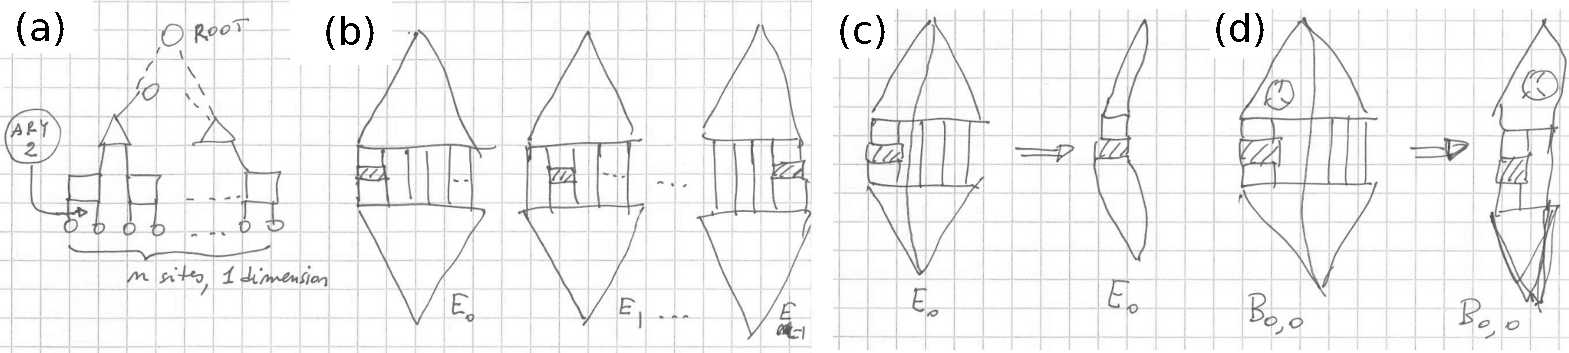
\includegraphics[clip,width=\textwidth]{figure1.png}%
\caption{(a) A MERA with ary 2, dimension 1, and $n$ sites as indicated.
	(b) All energies $E_l$ for $l=0,\cdots,n-1$ for a 2-local Hamiltonian shown as the tensor in shaded rectangles.
	(c) Causal cone simplification of $E_0$. (d) Causal cone simplification of $B_{0,0}$.}
\end{figure}

\section{Work Needed for the Symbolic Driver}
\begin{enumerate}
	\item Implement more geometries like dimension 3 hyper-rectangular, triangular lattices. Note that dimension 2 rectangular has already been implemented.
	Difficulty: medium to hard.
	\item Implement more arities like ternary MERA. Only binary MERA has been implemented so far. 	Difficulty: medium to hard.
	\item Implement more Models. Only Heisenberg spin one-half has been implemented so far. 	Difficulty: medium to hard for bosonic models, very hard for
	fermionic models.
	\item The symbolic driver \code{merapp} should be able to specify local symmetries. Difficulty level: hard.
	\item The symbolic driver should be able to handle fermionic models via ``diamond'' tensors: Difficult level: very hard.
\end{enumerate}
\end{document}
